
\section{Глава 1. Предметная область}

\subsection{Математическая модель квадрокоптера}
Для понимания принципов полета квадрокоптера рассмотрим его математическую модель в двух системах координат(СК):

1. Неподвижная система координат (НСК), в качестве которой выступает нормальная земная система координат с заданными перпендикулярными друг другу координатными осями \(O_{g}X_{g}\), \(O_{g}Y_{g}\), и \(O_{g}Z_{g}\), причем ось \(O_{g}Z_{g}\) направлена противоположно вектору силы тяжести.

2. Связанная с квадрокоптером система координат (ССК), центр которой размещен в центре масс аппарата, а оси \(OX\), \(OY\), и \(OZ\) параллельны и сонаправлены с осями неподвижной системы. Угловое положение аппарата зададим тремя углами Эйлера: углами крена \(\phi\), тангажа \(\theta\) и рыскания \(\psi]\), определяющими вращение вокруг осей OX, OY, и OZ соответственно. Основываясь на ранее рассмотренных системах координат можно утверждать о том, что квадрокоптер имеет шесть степеней свободы, а именно три линейных координаты \([x; y; z ]\) и три угловых \([\theta, \phi, \psi]\). В качестве управляющих каналов выступают скорости вращения роторов (рис. \ref{fig:ris1}), которые создают динамику движения БПЛА в пространстве. Возникающие в результате подачи управляющих воздействий силы и моменты пропорциональны квадрату угловых скоростей винтов \(\Omega^2\). Поэтому, для достижения желаемого режима работы БПЛА, необходимо связать совокупность управляющих воздействий со степенями свободы БПЛА, через уравнения связи, которые определяют основные режимы движения квадрокоптера в пространстве.
% ~\ref{fig:ris1}
\begin{figure}[H]
	\centering
	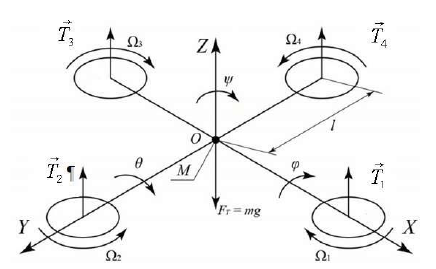
\includegraphics[width=0.5\linewidth]{../RW/pics/ris1}
	\caption{Связанная система координат квадрокоптера
	}
	\label{fig:ris1}
\end{figure}
В качестве первого режима БПЛА \(U_{1}\) рассмотрим движение вдоль оси \(OZ\), принадлежащей ССК. Данное движение обеспечивается одновременным увеличением скоростей винтов на одинаковое значение угловой скорости \(\Delta a\). Полученное при этом движение характеризуется взлетом или посадкой квадрокоптера (при нулевых значениях тангажа и крена) и описывается следующим выражением:
\begin{equation}
U_{1}=b(\Omega_{1}^2+\Omega_{2}^2+\Omega_{3}^2+\Omega_{4}^2)
\end{equation}
где \(b\) -- аэродинамическая составляющая тяги винта.
В качестве второго режима движения БПЛА \(U_{2}\) необходимо взять поворот вокруг оси \(OX\), принадлежащей ССК. Данное движение достигается путем увеличения/уменьшения на величину \(\Delta a\) значения \(\Omega_{4}\) левого винта и уменьшением/увеличением на величину \(\Delta b\) значения \(\Omega_{1}\)
правого. Полученное при этом движение характеризуется изменением угла крена \(\phi\) и описывается следующим выражением:
\begin{equation}
U_{2}=lb(-\Omega_{2}^2-\Omega_{4}^2)
\end{equation}
где \(l\) -- расстояние между центром квадрокоптера и центром винта.

В качестве третьего режима движения \(U_{3}\) необходимо взять поворот БПЛА вокруг оси \(OY\), принадлежащей ССК. Данное движение достигается путем уменьшения/увеличения на величину \(\Delta a\) значения \(\Omega_{1}\) фронтального винта и увеличения/уменьшения на величину \(\Delta b\) значения \(\Omega_{3}\) заднего. Полученное при этом движение характеризуется изменением угла тангажа \(\theta\) и описывается следующим выражением:
\begin{equation}
U_{3}=lb(-\Omega_{1}^2-\Omega_{3}^2)
\end{equation}

В качестве последнего, четвертого, режима движения \(U_{4}\) необходимо взять поворот БПЛА вокруг оси OZ, принадлежащей ССК. Данное движение достигается путем одновременного увеличения/уменьшения на величину \(\Delta a\) значений \(\Omega_{4}\) левого и \(\Omega_{2}\) правого винтов, а также одновременного уменьшения/увеличения на величину \(\Delta b\) значений \(\Omega_{1}\) фронтального и \(\Omega_{3}\) заднего винтов. Благодаря вращению роторов в диагонально противоположных направлениях, полученное движение характеризуется изменением угла рыскания \(\psi\) и описывается следующим выражением:
\begin{equation}
U_{4}=d(-\Omega_{1}^2+\Omega_{2}^2-\Omega_{3}^2+\Omega_{4}^2)
\end{equation}
где \(d\) -- аэродинамическая составляющая коэффициента сопротивления среды.
Введенное с учетом (1) -- (4) множество \(U\), характеризующее режимы
движения квадрокоптера, можно записать следующим образом:

\begin{equation}
U = \left\{ \begin{aligned}
U_{1}&=&b(\Omega_{1}^2+\Omega_{2}^2+\Omega_{3}^2+\Omega_{4}^2)\\
U_{2}&=&lb(-\Omega_{2}^2-\Omega_{4}^2)\\
U_{3}&=&lb(-\Omega_{1}^2-\Omega_{3}^2)\\
U_{4}&=&d(-\Omega_{1}^2+\Omega_{2}^2-\Omega_{3}^2+\Omega_{4}^2)
\end{aligned} \right.
\end{equation}

Множество \(U\) определяет связь между системой исполнительных приводов и платформой БПЛА \cite{mathmodel}.

\subsection{Устройство квадрокоптера}
Далее рассмотрим компонентную базу квадрокоптера.

Квадрокоптер -- беспилотный летательный аппарат мультироторного типа с четырьмя несущими ВМГ.
Квадрокоптер состоит из (условная схема представлена на):

--- рамы;

--- 4 моторов, пропеллеров (винто -- моторная группа, далее ВМГ);

--- 4 регуляторов оборотов (далее рассматривается как часть ВМГ);

--- полетного контроллера;

--- аккумулятора;

--- камеры, видеопередатчика, видеоантенны (опционально для FPV);

--- радиоприемника (радиопередатчика, если необходима отправка телеметрии);

--- другой периферии (например, GPS, магнитометр, дальномер, телеметрийный модуль).

 % ~\ref{fig:pix}
 \begin{figure}[H]
 	\centering
 	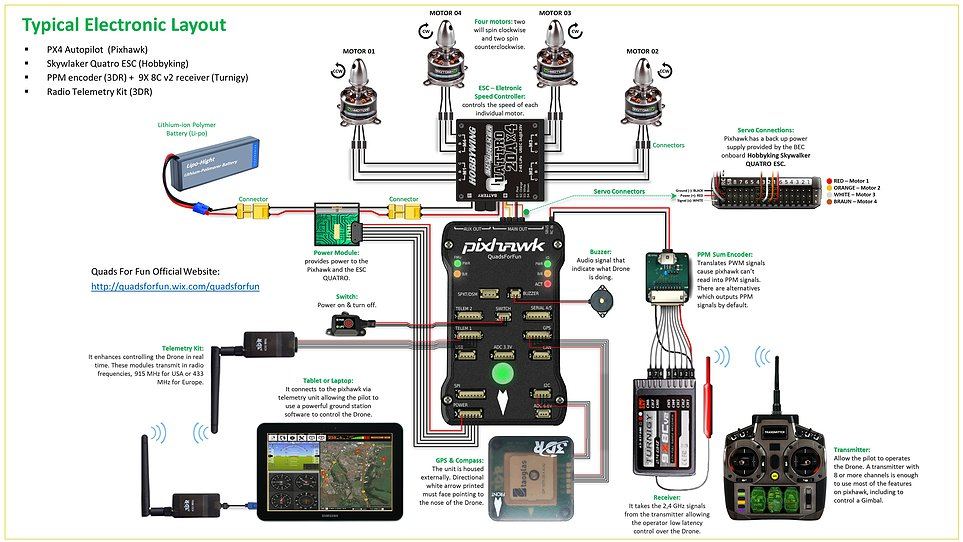
\includegraphics[width=0.5\linewidth]{../RW/pics/pix}
 	\caption{Пример схемы подключения
 	}
 	\label{fig:pix}
 \end{figure}
Рассмотрим каждый компонент с его характеристиками подробнее.

%винты должжны вмещаться и не создавать турбулентный поток
Рама - несущий компонент, на котором располагается вся электроника квадрокоптера. Рама должна быть жесткой, прочной, и в то же время легкой. На данный момент лучшим материалом для рам квадрокоптеров является карбон.

Компоненты ВМГ подбираются в зависимости от поставленных задач и характеристик БПЛА. Для современных БПЛА используются моторы бесколлекторного типа. Основными их характеристиками являются размер и количество оборотов на вольт.
Диаметр, шаг и количество лопастей пропеллера определяют тягу квадрокоптера. При этом пропеллеры с большим шагом обеспечивают большую скорость полета.

Регулятор принимает управляющий сигнал с полетного контроллера и на его основе задает обороты моторов. В случае мотора бесколлекторного типа это происходит путем открытия силовых ключей (мосфетов) для коммутации обмоток.

Полетный контроллер -- система реального времени, которая интерпретирует входящие данные от приемника и бортовых датчиков (гироскопа, акселерометра, барометра и др.), на основе которых рассчитывает положение квадрокоптера и производит регулирование путем выдачи управляющего сигнала на ВМГ. Все алгоритмы работы полетного контроллера содержатся в прошивке -- программном обеспечении, которое выбирается в зависимости от схемы полетного контроллера и поставленных задач.

Для питания квадрокоптера используются литий-полимерные и литий-ионные аккумуляторы. В зависимости от задач и размеров подбирается количество ячеек аккумулятора, емкость и токоотдача.

Видеосистема состоит из трех основных компонентов: камера, видеопередатчик, приемник, передающая и принимающая антенны. Видеопередатчик, в большинстве случаев, функционирует на диапазоне частот 5.8 ГГц.

Для осуществления контроля над квадрокоптером используется радиоуправление. Для приема сигнала к полетному контроллеру подключается приемник, общающийся с передатчиком по определенному протоколу на указанном диапазоне частот. Информация с датчиков квадрокоптера оператору может передаваться с помощью устройств приема-передачи телеметрии.

Также на квадрокоптер ставится бортовой компьютер для выполнения более высокоуровневых вычислительных задач, например, когда необходима обработка видеопотока или выполнение других высокоуровневых вычислительных задач. Как правило, бортовой компьютер представляет собой микрокомпьютер, например, Ras\-pber\-ry Pi или Nvi\-dia Jet\-son. 

Теперь разберем, какие есть прошивки для полетных контроллеров.

\subsection{Семейства прошивок полетного контроллера}
Ввиду того, что нам может потребоваться доработка функционала прошивки полетного контроллера, мы не будем рассматривать прошивки с закрытым исходным кодом. Наряду с функционалом прошивки одним из ключевых факторов ее выбора будет тип открытой лицензии. Если взять во внимание наиболее популярные открытые прошивки для полетных контроллеров, то можно выделить 2 семейства: потомки MultiWii и прошивки под полетные контроллеры семейства PixHawk.

MultiWii - прошивка, изначально разработанная для получения и обработки данных с гироскопов и акселерометров игровой консоли Nintendo Wii. Позже, на основе частей из консоли Nintendo Wii (акселерометр + гироскоп) и контроллера atmega, был спроектирован полетный контроллер, на который была установлена уже коптерная прошивка MultiWii \cite{multiwii}. Со временем платформа atmega перестала удовлетворять аппаратным критериям, и MultiWii перерос в BaseFlight, базирующийся на чипах семейства STM32, а он в свою очередь в CleanFlight. Разработчики CleanFlight разошлись во мнениях касаемо функционала прошивки и сделали следующие ответвления:

---BetaFlight;

---INav;

---EmuFlight.

BetaFlight нацелен на гоночные квадрокоптеры. Основными особенностями являются: минимальная фазовая задержка, точное следование управляющему сигналу (setpoint) и поддержка огромного количества полетных контроллеров (target).
Стоит пояснить фразу "минимальная фазовая задержка". При фильтрации показаний гироскопа происходит сдвиг по фазе между исходным и фильтрованным сигналами, что приводит к запозданию реакции ПИД регулятора, и как итог -- ПИД осцилляции. Фильтры в BetaFlight оптимизированы для уменьшения фазовой задержки.

INav сфокусирован на навигационных возможностях. Позволяет выполнять полеты по точкам, исходя из данных, полученных периферией. Поддерживает различные платформы, включая БПЛА мультироторного и самолетного типов, сухопутные и водные управляемые модели.

EmuFlight предназначен для акробатических и кинематографических полетов. Позволяет настроить квадрокоптер на плавный полет, содержит множество алгоритмов для фильтрации шумов.

Среди описанных прошивок только INav имеет функционал для автономных полетов, но инструменты внешнего управления имеют весьма скудный функционал, потому такой вариант не подходит для решения поставленной задачи.

В семействе полетных контроллеров PixHawk наиболее популярны прошивки PX4 и Ardupilot. Эти прошивки активно используются как хоббистами, так и для решения профессиональных задач в промышленности и сфере эксплуатации БАС. Практически весь их функционал нацелен на выполнение автономных миссий. Ardupilot, в основном, разрабатывается и используется хоббийным сообществом. PX4 изначально был студенческой учебно-исследовательской работой, но сейчас его используют исследователи в области программирования, стабилизации и навигации БПЛА во всем мире.

Изначально это был студенческий НИР, но спустя 3 года вышел официальный релиз, сейчас его используют исследователи в области программирования, стабилизации и навигации БПЛА во всем мире. Главными особенностями PX4 являются поддержка огромного количества датчиков и навигация в режиме OFFBOARD, который позволяет управлять беспилотником при помощи бортового компьютера. OFFBOARD режим PX4 предоставляет огромные возможности для конфигурирования и управления полетным заданием с внешнего устройства, что подходит для поставленной задачи. Рассмотрим PX4 подробнее.

\subsection{PX4}
%\url{https://docs.px4.io/master/en/getting_started/px4_basic_concepts.html}
%\url{https://docs.px4.io/master/en/contribute/licenses.html}
%https://docs.px4.io/master/en/simulation/#simulator-mavlink-api

PX4 - прошивка с открытым исходным кодом, публикуемая под лицензией BSD-3-Clause. PX4 позволяет управлять различными типами беспилотников, включая: летательные (мультикоптеры, самолеты и вертолеты), наземные и подводные аппараты. Он совместим с большим количеством оборудования, датчиков и другой периферии. Позволяет реализовать гибкие режимы полета и функции безопасности.
Параметры PX4 настраиваются с помощью Q\-Ground\-Control \cite{px4}.

QGroundControl - кросплатформенный конфигуратор для настройки PX4 и Ardupilot прошивок. Он обеспечивает полное управление полетом и настройку беспилотника \cite{qgroundcontrol}.

PX4 для определения состояния аппарата, его стабилизации и автономного полета использует датчики, такие как: гироскоп, акселерометр, магнитометр (компас) и барометр. Для включения всех автоматических режимов и некоторых вспомогательных требуется GPS или другая система позиционирования.
Для передачи данных / телеметрии между наземной станцией управления, такой как Q\-Ground\-Control, и беспилотником, работающим под управлением PX4 может использоваться как проводное, так и беспроводное соединение по протоколу MAVLink. Он позволяет настраивать параметры во время полета, проверять телеметрию в режиме реального времени, менять миссию на лету и т. д.

PX4 можно управлять с отдельного компьютера через кабель или Wi-Fi. Дрон и компьютер обычно обмениваются данными с помощью API MAVLink, такого как MAVSDK или MAVROS \cite{px4}.

\subsection{MAVLink}

%\url{https://mavlink.io/en/}

MAVLink -- это протокол двоичной телеметрии, разработанный для систем с ограниченными ресурсами и каналов с ограниченной пропускной способностью. MAVLink был впервые выпущен в начале 2009 года Лоренцем Мейером (основателем PX4) и в настоящее время имеет значительное количество разработчиков. Протокол развернут в двух основных версиях: v1.0 и v2.0, которые имеют обратную совместимость (реализации v2.0 могут анализировать и отправлять пакеты v1.0).

MAVLink реализует гибрид шаблонов проектирования взаимодействия «публикация -- подписка» и «точка -- точка». В этом гибридном шаблоне потоки данных отправляются / публикуются как темы, а подпротоколы конфигурации, такие как протокол задания или протокол параметров, реализуются шаблоном «точка-точка» с повторной передачей.

Сообщения определяются в файлах XML. Каждый файл XML определяет набор сообщений, поддерживаемый MAVLink системой, также называемый «диалектом». Набор эталонных сообщений, который реализуется большинством наземных станций управления и автопилотов, определен в common.xml (большинство диалектов основано на этом определении).

Набор инструментов MAVLink использует определения XML сообщений для генерации библиотеки MAVLink для каждого из поддерживаемых языков программирования . Дроны, наземные станции управления и другие системы MAVLink используют сгенерированные библиотеки для связи. Они распространяются под лицензией MIT и поэтому могут использоваться без ограничений в любом приложении с закрытым исходным кодом без публикации исходного кода. MAVLink был впервые выпущен в начале 2009 года Лоренцем Мейером (основателем PX4) и в настоящее время имеет значительное количество разработчиков \cite{px}.

MAVLink поддерживает множество языков программирования, работающих на множестве микроконтроллеров / операционных систем (включая ARM7, ATMega, dsPic, STM32 и Windows, Linux, MacOS, Android и iOS). Допускает одновременно до 255 систем в сети (беспилотники, наземные станции и т. д.)

Обеспечивает как внешнюю, так и бортовую связь (например, между q\-ground\-con\-trol и дроном, а также между автопилотом дрона и камерой дрона с поддержкой MAVLink) \cite{mavlink}.

MAVLink развернут в двух основных версиях: v1.0 и v2.0, которые имеют обратную совместимость (реализации v2.0 могут анализировать и отправлять пакеты v1.0). Потоки телеметрических данных отправляются в многоадресном режиме, в то время как аспекты протокола, которые изменяют конфигурацию системы и требуют гарантированной доставки, являются point-to-point с повторной передачей.

%//переделать

Для того, чтобы запускать на наземной станции автономные миссии для БПЛА, необходим набор инструментов, позволяющий обрабатывать MAVLink сообщения, преобразовывать показания с камеры в координаты положения квадрокоптера и отправлять управляющие команды квадрокоптеру. Для выполнения обозначенного функционала можно использовать робототехнические фреймворки. Наиболее популярным робототехническим фреймворком является ROS.
% дописать про офборд
\subsection{Robotic Operating System}
%\url{https://www.ros.org/about-ros/}

Robotic Operating System (далее ROS) -- это гибкая платформа для написания программного обеспечения для роботов; набор инструментов, библиотек и соглашений, которые призваны упростить задачу создания сложного и надежного поведения роботов на самых разных роботизированных платформах \cite{ros}.

Целью создания ROS является создание среды разработки, которая позволяет разработчикам ПО для роботов взаимодействовать на глобальном уровне.

ROS сосредоточена на максимизации повторного использования кода при разработке. Основные характеристики, позволяющие это реализовать:

Распределенные процессы. Структура ROS создана в виде минимальных единиц исполняемых процессов (нод), и каждый процесс выполняется изолированно. Взаимодействие разных нод происходит только на уровне обмена сообщениями.

Управление пакетами. Несколько процессов, имеющих общую задачу, объединяются в пакеты. Управление пакетами подразумевает набор утилит, позволяющих автоматически скачивать, устанавливать и удалять пакеты. Пакетный менеджер гарантирует работоспособность и целостность установленных пакетов.

Публичные репозитории и документация. Каждый доступный пакет публикуется в публичном репозитории. Документация пакетов публикуется в единой системе, которая упрощает поиск необходимых пакетов.

Единое API. При разработке программы, использующей ROS, вы получаете простое и легко встраиваемое API. При этом при использовании API нет разницы, на каком языке была написана программа.

Поддержка различных языков программирования. ROS предоставляет клиентские библиотеки для поддержки различных языков программирования. Наиболее популярны Python, C ++, а также такие языки, как Lisp, JAVA, C\#, Lua и Ruby \cite{voltbro}.


Концепции ROS.

Ноды.

ROS-нода – это специальная программа (обычно написанная на Python или C++), которая взаимодействует с другими нодами посредством ROS-топиков и ROS-сервисов. Разделение сложных робототехнических систем на изолированные ноды дает определенные преимущества: понижается связанность кода, повышается переиспользуемость и надежность.

Очень многие робототехнические библиотеки и драйвера выполнены именно в виде ROS-нод.

Для того, чтобы превратить обычную программу в ROS-ноду, необходимо подключить к ней библиотеку rospy или roscpp и добавить инициализирующий код.

Пример ROS-ноды на языке Python:

\begin{Program}[H]
	\caption{Пример ROS-ноды на языке Python:} \label{lst:1}
	\begin{MyCode}
import rospy

rospy.init\_node('my\_ros\_node')  # имя ROS-ноды

rospy.spin()  # входим в бесконечный цикл...
	\end{MyCode}
\end{Program}
Топики.

Топик – это именованная шина данных, по которой ноды обмениваются сообщениями. Любая нода может опубликовать сообщение в произвольный топик, а также подписаться на произвольный топик.

\begin{Program}[H]
	\caption{Пример публикации сообщения типа std\_msgs/String (строка) в топик foo на языке Python:} \label{lst:2}
	\begin{MyCode}
from std_msgs.msg import String

# создаем Publisher'а
foo_pub = rospy.Publisher('/foo', String, queue_size=1)

# публикуем сообщение
foo_pub.publish(data='Hello, world!')
	\end{MyCode}
\end{Program}
\begin{Program}[H]
	\caption{Пример подписки на топик /foo на языке Python:} \label{lst:3}
	\begin{MyCode}
def foo_callback(msg):
print msg.data

#При получении сообщения в топик /foo будет вызвана функция foo\_callback.
rospy.Subscriber('/foo', String, foo_callback)
	\end{MyCode}
\end{Program}

Также существует возможность работы с топиками с помощью утилиты rostopic. Например, с помощью следующей команды можно просматривать сообщения, публикуемые в топик /mavros/state:

rostopic echo /mavros/state

Сервисы.

Сервис – это некоторый аналог функции, которая может быть вызвана из одной ноды, а обработана в другой. У сервиса есть имя, аналогичное имени топика, и 2 типа сообщений: тип запроса и тип ответа \cite{clover}.

\begin{Program}[H]
	\caption{Пример вызова ROS-сервиса из языка Python:} \label{lst:4}
	\begin{MyCode}
from clover.srv import GetTelemetry

# Создаем обертку над сервисом get\_telemetry пакета clover с типом GetTelemetry:
get_telemetry = rospy.ServiceProxy('get_telemetry', srv.GetTelemetry)

# Вызываем сервис и получаем телеметрию квадрокоптера:
telemetry = get_telemetry()
# С сервисами можно также работать при помощи утилиты rosservice.
# Так можно вызвать сервис /get_telemetry из командной строки:

rosservice call /get\_telemetry "{frame_id: ''}"
	\end{MyCode}
\end{Program}


\subsection{MAVROS}
%\url{https://clover.coex.tech/ru/mavros.html}
%\url{https://dev.px4.io/master/en/ros/mavros\_installation.html}
Так как мы выбрали ROS как основной фреймворк для реализации нашего решения и MAVLink, в качестве основного протокола -- нам необходим компонент, обеспечивающий взаимодействие обозначенных систем.
MAVROS (MAVLink + ROS) -- это пакет для ROS, предоставляющий возможность управлять беспилотниками по протоколу MAVLink. MAVROS поддерживает полетные стеки PX4 и APM. Связь организовывается по UART, USB, TCP или UDP.

MAVROS подписывается на определенные ROS-топики в ожидании команд, публикует в другие топики телеметрию, и предоставляет сервисы.
Пакет mavros обеспечивает расширяемую связь MAVLink между компьютерами, на которых работает ROS, автопилоты с поддержкой MAVLink и GCS с поддержкой MAVLink. Нода MAVROS запускается в launch-файле \cite{clover}.

MAVROS -- это «официальный» поддерживаемый мост между ROS и протоколом MAVLink. В настоящее время он расширяется, чтобы включить обмен сообщениями fast-RTPS, включая уровень для преобразования сообщений uORB PX4 в общие идиомы ROS.

Эти расширения в последующем могут существенно улучшить скорость работы разрабатываемого решения.
%https://dev.px4.io/v1.9.0/en/setup/fast-rtps-installation.html доработать